\documentclass[12pt]{amsart}
\usepackage[utf8]{inputenc}
\usepackage{amsfonts, amssymb, latexsym, graphicx, hyperref, amsmath}
%\usepackage[linesnumbered,ruled]{algorithm2e}
\usepackage{tikz}
\title{rothe-diagram-template}
\date{October 2019}
\begin{document}
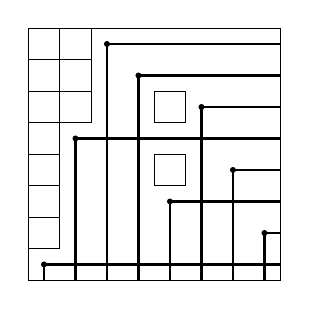
\begin{tikzpicture}[scale=.4]
\draw (0,0) rectangle (8,8);
\filldraw (2.5,7.5) circle (.5ex);
\draw[line width = .2ex] (2.5,0) -- (2.5,7.5) -- (8,7.5);
\draw (0, 7) rectangle (1,8);
\draw (1, 7) rectangle (2,8);
\filldraw (3.5,6.5) circle (.5ex);
\draw[line width = .2ex] (3.5,0) -- (3.5,6.5) -- (8,6.5);
\draw (0, 6) rectangle (1,7);
\draw (1, 6) rectangle (2,7);
\filldraw (5.5,5.5) circle (.5ex);
\draw[line width = .2ex] (5.5,0) -- (5.5,5.5) -- (8,5.5);
\draw (0, 5) rectangle (1,6);
\draw (1, 5) rectangle (2,6);
\draw (4, 5) rectangle (5,6);
\filldraw (1.5,4.5) circle (.5ex);
\draw[line width = .2ex] (1.5,0) -- (1.5,4.5) -- (8,4.5);
\draw (0, 4) rectangle (1,5);
\filldraw (6.5,3.5) circle (.5ex);
\draw[line width = .2ex] (6.5,0) -- (6.5,3.5) -- (8,3.5);
\draw (0, 3) rectangle (1,4);
\draw (4, 3) rectangle (5,4);
\filldraw (4.5,2.5) circle (.5ex);
\draw[line width = .2ex] (4.5,0) -- (4.5,2.5) -- (8,2.5);
\draw (0, 2) rectangle (1,3);
\filldraw (7.5,1.5) circle (.5ex);
\draw[line width = .2ex] (7.5,0) -- (7.5,1.5) -- (8,1.5);
\draw (0, 1) rectangle (1,2);
\filldraw (0.5,0.5) circle (.5ex);
\draw[line width = .2ex] (0.5,0) -- (0.5,0.5) -- (8,0.5);
\end{tikzpicture}

\newline
\vspace{1.0cm}

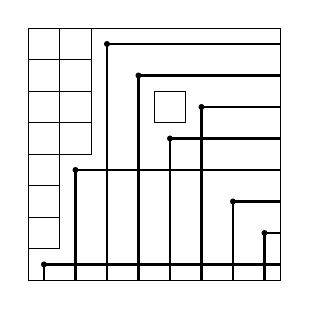
\begin{tikzpicture}[scale=.4]
\draw (0,0) rectangle (8,8);
\filldraw (2.5,7.5) circle (.5ex);
\draw[line width = .2ex] (2.5,0) -- (2.5,7.5) -- (8,7.5);
\draw (0, 7) rectangle (1,8);
\draw (1, 7) rectangle (2,8);
\filldraw (3.5,6.5) circle (.5ex);
\draw[line width = .2ex] (3.5,0) -- (3.5,6.5) -- (8,6.5);
\draw (0, 6) rectangle (1,7);
\draw (1, 6) rectangle (2,7);
\filldraw (5.5,5.5) circle (.5ex);
\draw[line width = .2ex] (5.5,0) -- (5.5,5.5) -- (8,5.5);
\draw (0, 5) rectangle (1,6);
\draw (1, 5) rectangle (2,6);
\draw (4, 5) rectangle (5,6);
\filldraw (4.5,4.5) circle (.5ex);
\draw[line width = .2ex] (4.5,0) -- (4.5,4.5) -- (8,4.5);
\draw (0, 4) rectangle (1,5);
\draw (1, 4) rectangle (2,5);
\filldraw (1.5,3.5) circle (.5ex);
\draw[line width = .2ex] (1.5,0) -- (1.5,3.5) -- (8,3.5);
\draw (0, 3) rectangle (1,4);
\filldraw (6.5,2.5) circle (.5ex);
\draw[line width = .2ex] (6.5,0) -- (6.5,2.5) -- (8,2.5);
\draw (0, 2) rectangle (1,3);
\filldraw (7.5,1.5) circle (.5ex);
\draw[line width = .2ex] (7.5,0) -- (7.5,1.5) -- (8,1.5);
\draw (0, 1) rectangle (1,2);
\filldraw (0.5,0.5) circle (.5ex);
\draw[line width = .2ex] (0.5,0) -- (0.5,0.5) -- (8,0.5);
\end{tikzpicture}

\newline
\vspace{1.0cm}

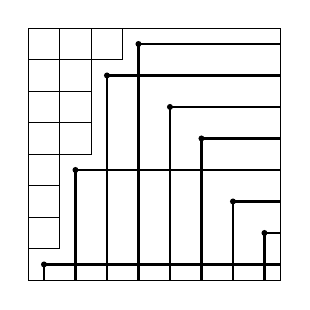
\begin{tikzpicture}[scale=.4]
\draw (0,0) rectangle (8,8);
\filldraw (3.5,7.5) circle (.5ex);
\draw[line width = .2ex] (3.5,0) -- (3.5,7.5) -- (8,7.5);
\draw (0, 7) rectangle (1,8);
\draw (1, 7) rectangle (2,8);
\draw (2, 7) rectangle (3,8);
\filldraw (2.5,6.5) circle (.5ex);
\draw[line width = .2ex] (2.5,0) -- (2.5,6.5) -- (8,6.5);
\draw (0, 6) rectangle (1,7);
\draw (1, 6) rectangle (2,7);
\filldraw (4.5,5.5) circle (.5ex);
\draw[line width = .2ex] (4.5,0) -- (4.5,5.5) -- (8,5.5);
\draw (0, 5) rectangle (1,6);
\draw (1, 5) rectangle (2,6);
\filldraw (5.5,4.5) circle (.5ex);
\draw[line width = .2ex] (5.5,0) -- (5.5,4.5) -- (8,4.5);
\draw (0, 4) rectangle (1,5);
\draw (1, 4) rectangle (2,5);
\filldraw (1.5,3.5) circle (.5ex);
\draw[line width = .2ex] (1.5,0) -- (1.5,3.5) -- (8,3.5);
\draw (0, 3) rectangle (1,4);
\filldraw (6.5,2.5) circle (.5ex);
\draw[line width = .2ex] (6.5,0) -- (6.5,2.5) -- (8,2.5);
\draw (0, 2) rectangle (1,3);
\filldraw (7.5,1.5) circle (.5ex);
\draw[line width = .2ex] (7.5,0) -- (7.5,1.5) -- (8,1.5);
\draw (0, 1) rectangle (1,2);
\filldraw (0.5,0.5) circle (.5ex);
\draw[line width = .2ex] (0.5,0) -- (0.5,0.5) -- (8,0.5);
\end{tikzpicture}

\newline
\vspace{1.0cm}

\end{document}